
%

\section{Explanation}
The general form of equation representing a pair of straight lines is 
\begin{align}
    ax^2+2bxy+cy^2+2dx+2ey+f=0
\end{align}
This can be represented as
\begin{align}
    \vec{x}^T\vec{V}\vec{x}+2\vec{u}^T\vec{x}+f=0\\
    \text{where, } \vec{V}=\myvec{a&b\\b&c}\\ \vec{u}=\myvec{d\\e}
\end{align}
This represents a pair of straight lines if
\begin{align}
    \mydet{\vec{V}&\vec{u}\\\vec{u}^T&f}=0
\end{align}
\section{Solution}
\mydet{\vec{V}&\vec{u}\\\vec{u}^T&f} of (1.0.1) becomes
\begin{align}
    \mydet{-3&-4&-\frac{29}{2}\\-4&3&\frac{3}{2}\\-\frac{29}{2}&\frac{3}{2}&-18}
\end{align}
Expanding equation (3.0.1), we get zero.\\
Hence given equation represents a pair of straight lines.
\section{Finding the individual lines}
Slopes of the individual lines are roots of equation 
\begin{align}
    cm^2+2bm+a=0\\
    \implies 3m^2-8m-3=0\\
    \text{Solving, }m=3,-\frac{1}{3}
\end{align}
The normal vectors of the lines then become
\begin{align}
    \vec{n_1}=\myvec{\frac{1}{3}\\1}\\
    \vec{n_2}=\myvec{-3\\1}
\end{align}
Equations of the lines can therefore be written as
\begin{align}
  \myvec{\frac{1}{3}&1}\vec{x}=c\\
 \implies \myvec{1&3}\vec{x}=c_1 ,\\
   \myvec{-3&1}\vec{x}=c_2\\
  \implies \left[\myvec{1&3}\vec{x}-c_1\right]\left[\myvec{-3&1}\vec{x}-c_2\right]
\end{align}
represents the equation specified in (1.0.1)\\
Comparing the equations, we have
\begin{align}
    \myvec{1&-3\\3&1}\myvec{c_2\\c_1}=\myvec{29\\-3}\\
 \end{align}
 Row reducing the augmented matrix
 \begin{align}
    \myvec{1&-3&29\\3&1&-3}\xleftrightarrow[]{R_2\leftarrow R_2-3\times R_1}
    \myvec{1&-3&29\\0&10&-90}\\
    \xleftrightarrow[]{R_2\leftarrow R_2\times \frac{1}{10}}
    \myvec{1&-3&29\\0&1&-9}\\
    \xleftrightarrow[]{R_1\leftarrow R_1+3\times R_2}
    \myvec{1&0&2\\0&1&-9}\\
    \implies c_2=2 \text{ and }c_1=-9
\end{align}
The individual line equations therefore become
\begin{align}
    \myvec{1&3}\vec{x}=-9 ,\\\myvec{-3&1}\vec{x}=2\\
    \implies 
    x+3y+9=0\\-3x+y-2=0
\end{align}
\section{Intersection Point}
The augmented matrix for the set of equations represented in (4.0.16), (4.0.17) is
\begin{align}
\myvec{1&3&-9\\-3&1&2}
\end{align}
Row reducing the matrix
\begin{align}
 \myvec{1&3&-9\\-3&1&2}\xleftrightarrow[]{R_2\leftarrow R_2+3\times R_1}\myvec{1&3&-9\\0&10&-25}\\
 \xleftrightarrow[]{R_1\leftarrow R_1-\frac{3}{10}\times R_2}\myvec{1&0&-\frac{3}{2}\\0&10&-25}\\
 \xleftrightarrow[]{R_2\leftarrow \frac{R_2}{10}}\myvec{1&0&-\frac{3}{2}\\0&1&-\frac{5}{2}}\\
\text{Hence, the intersection point is}
\myvec{-\frac{3}{2}\\-\frac{5}{2}}
\end{align}
\begin{figure}[!ht]
\centering
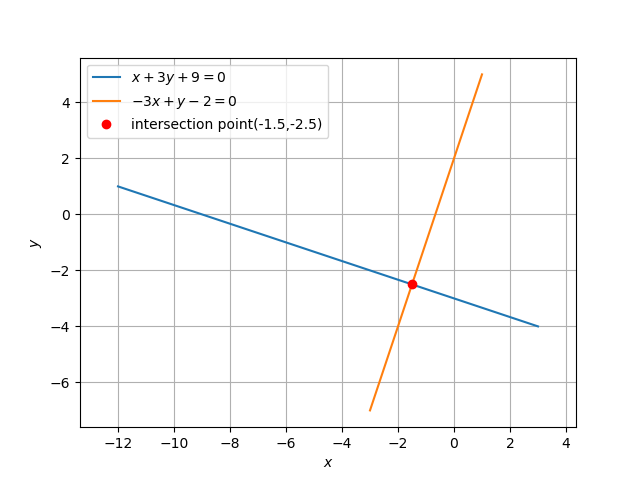
\includegraphics[width=\columnwidth]{hw4plot.png}
\caption{plot showing intersection of lines}
\label{Fig}
\end{figure}
\newpage
\section{Angle Between The Lines}
Angle between two lines $\theta$ can be given by
\begin{align}
\cos \theta = \frac{\vec{n_1}^T\vec{n_2}}{\norm{\vec{n_1}}\norm{\vec{n_2}}}
\end{align}
From (4.0.16), (4.0.17),
\begin{align}
\cos \theta=\frac{\myvec{1&3}\myvec{-3\\1}}{\sqrt{(3)^2 +1} \times \sqrt{(-3)^2 +1}}=0\\
\implies \theta = 90\degree
\end{align}
\end{document}

